\documentclass[10pt, a4paper, english]{article}\usepackage[]{graphicx}\usepackage[dvipsnames]{xcolor}
% maxwidth is the original width if it is less than linewidth
% otherwise use linewidth (to make sure the graphics do not exceed the margin)
\makeatletter
\def\maxwidth{ %
  \ifdim\Gin@nat@width>\linewidth
    \linewidth
  \else
    \Gin@nat@width
  \fi
}
\makeatother

\definecolor{fgcolor}{rgb}{0.345, 0.345, 0.345}
\newcommand{\hlnum}[1]{\textcolor[rgb]{0.686,0.059,0.569}{#1}}%
\newcommand{\hlstr}[1]{\textcolor[rgb]{0.192,0.494,0.8}{#1}}%
\newcommand{\hlcom}[1]{\textcolor[rgb]{0.678,0.584,0.686}{\textit{#1}}}%
\newcommand{\hlopt}[1]{\textcolor[rgb]{0,0,0}{#1}}%
\newcommand{\hlstd}[1]{\textcolor[rgb]{0.345,0.345,0.345}{#1}}%
\newcommand{\hlkwa}[1]{\textcolor[rgb]{0.161,0.373,0.58}{\textbf{#1}}}%
\newcommand{\hlkwb}[1]{\textcolor[rgb]{0.69,0.353,0.396}{#1}}%
\newcommand{\hlkwc}[1]{\textcolor[rgb]{0.333,0.667,0.333}{#1}}%
\newcommand{\hlkwd}[1]{\textcolor[rgb]{0.737,0.353,0.396}{\textbf{#1}}}%
\let\hlipl\hlkwb

\usepackage{framed}
\makeatletter
\newenvironment{kframe}{%
 \def\at@end@of@kframe{}%
 \ifinner\ifhmode%
  \def\at@end@of@kframe{\end{minipage}}%
  \begin{minipage}{\columnwidth}%
 \fi\fi%
 \def\FrameCommand##1{\hskip\@totalleftmargin \hskip-\fboxsep
 \colorbox{shadecolor}{##1}\hskip-\fboxsep
     % There is no \\@totalrightmargin, so:
     \hskip-\linewidth \hskip-\@totalleftmargin \hskip\columnwidth}%
 \MakeFramed {\advance\hsize-\width
   \@totalleftmargin\z@ \linewidth\hsize
   \@setminipage}}%
 {\par\unskip\endMakeFramed%
 \at@end@of@kframe}
\makeatother

\definecolor{shadecolor}{rgb}{.97, .97, .97}
\definecolor{messagecolor}{rgb}{0, 0, 0}
\definecolor{warningcolor}{rgb}{1, 0, 1}
\definecolor{errorcolor}{rgb}{1, 0, 0}
\newenvironment{knitrout}{}{} % an empty environment to be redefined in TeX

\usepackage{alltt}
%typesetting
\usepackage[margin = 1in]{geometry} % margins
\usepackage[T1]{fontenc} % font encoding
\usepackage{babel} %enables typesetting for multiple languages
\usepackage{parskip} %new lines
\usepackage{graphicx} 
\usepackage{float}
\floatplacement{figure}{H} %when printing tables, include  table.position="H"
\usepackage{bm}
\usepackage{amsmath}

\usepackage[dvipsnames]{xcolor} % more colors

\usepackage[colorlinks]{hyperref}


 %clickable table of contents from hyperref
\hypersetup{
    colorlinks,
    citecolor=black,
    filecolor=black,
    linkcolor=black,
    urlcolor=black
}

\usepackage[colorinlistoftodos]{todonotes}
\setcounter{secnumdepth}{0}

\title{Machine Learning 2ST129 26605 HT2023
 Assignment 7}
\author{Anonymous Student}
\date{\today}
\IfFileExists{upquote.sty}{\usepackage{upquote}}{}
\begin{document}
\maketitle
\newpage
\tableofcontents
\newpage

\section{General Information}
\begin{itemize}
\item Time used for reading: 3 hours  
\item Time used for basic assignment: 16 hours
\item Time used for extra assignment: NA
\item Good with lab: I think that in general it was a good overall structure of the different tasks. For example, that we had to implement something, plot it and also interpret it, which I felt was good for learning.
\item Things improve with lab: In my opinion, it would have been good if there was some more information about the code, especially for task 1. For example, now I mostly copy pasted the code from the linked guide to get it to work, but I do not really know what some of that parts are supposed to represent. 
\end{itemize}

\newpage


\section{Task 1}

\subsection{1.1}
First we load the required libraries as well as the mnist data
\begin{knitrout}
\definecolor{shadecolor}{rgb}{0.969, 0.969, 0.969}\color{fgcolor}\begin{kframe}
\begin{alltt}
\hlcom{#Libraries}
 \hlkwd{library}\hlstd{(tidyverse)}
 \hlkwd{library}\hlstd{(xtable)}
 \hlkwd{library}\hlstd{(tensorflow)}
 \hlkwd{library}\hlstd{(keras)}
\end{alltt}
\end{kframe}
\end{knitrout}

\begin{knitrout}
\definecolor{shadecolor}{rgb}{0.969, 0.969, 0.969}\color{fgcolor}\begin{kframe}
\begin{alltt}
\hlstd{mnist} \hlkwb{<-} \hlkwd{dataset_mnist}\hlstd{()}
\hlstd{x_train} \hlkwb{<-} \hlstd{mnist}\hlopt{$}\hlstd{train}\hlopt{$}\hlstd{x}\hlopt{/}\hlnum{255}
\hlstd{x_test} \hlkwb{<-} \hlstd{mnist}\hlopt{$}\hlstd{test}\hlopt{$}\hlstd{x}\hlopt{/}\hlnum{255}
\hlstd{x_train} \hlkwb{<-} \hlkwd{array_reshape}\hlstd{(x_train,} \hlkwd{c}\hlstd{(}\hlkwd{nrow}\hlstd{(x_train),} \hlnum{784}\hlstd{),} \hlkwc{order} \hlstd{=} \hlstr{"F"}\hlstd{)}
\hlstd{x_test} \hlkwb{<-} \hlkwd{array_reshape}\hlstd{(x_test,} \hlkwd{c}\hlstd{(}\hlkwd{nrow}\hlstd{(x_test),} \hlnum{784}\hlstd{),} \hlkwc{order} \hlstd{=} \hlstr{"F"}\hlstd{)}
\end{alltt}
\end{kframe}
\end{knitrout}


\subsection{1.2}
Now we want to implement a a one-layer (encoder and decoder) feed-forward variational autoencoder with two latent dimensions such that both the encoder and decoder layers should each have 200 hidden units. The following code is pretty much all based on the example as provided by the variational\_autoencoder.R guide on GitHub. Though with some minor differences such that we change the dimensions.  



\begin{knitrout}
\definecolor{shadecolor}{rgb}{0.969, 0.969, 0.969}\color{fgcolor}\begin{kframe}
\begin{alltt}
\hlkwa{if} \hlstd{(tensorflow}\hlopt{::}\hlstd{tf}\hlopt{$}\hlkwd{executing_eagerly}\hlstd{())}
  \hlstd{tensorflow}\hlopt{::}\hlstd{tf}\hlopt{$}\hlstd{compat}\hlopt{$}\hlstd{v1}\hlopt{$}\hlkwd{disable_eager_execution}\hlstd{()}
\hlstd{batch_size} \hlkwb{<-} \hlnum{100L}
\hlstd{original_dim} \hlkwb{<-} \hlnum{784L}
\hlstd{latent_dim} \hlkwb{<-} \hlnum{2L}
\hlstd{intermediate_dim} \hlkwb{<-} \hlnum{200L}
\hlstd{epochs} \hlkwb{<-} \hlnum{50L}
\hlstd{epsilon_std} \hlkwb{<-} \hlnum{1.0}

\hlcom{# Model definition --------------------------------------------------------}

\hlstd{x} \hlkwb{<-} \hlkwd{layer_input}\hlstd{(}\hlkwc{shape} \hlstd{=} \hlkwd{c}\hlstd{(original_dim))}
\hlstd{h} \hlkwb{<-} \hlkwd{layer_dense}\hlstd{(x, intermediate_dim,} \hlkwc{activation} \hlstd{=} \hlstr{"relu"}\hlstd{)}
\hlstd{z_mean} \hlkwb{<-} \hlkwd{layer_dense}\hlstd{(h, latent_dim)}
\hlstd{z_log_var} \hlkwb{<-} \hlkwd{layer_dense}\hlstd{(h, latent_dim)}

\hlstd{sampling} \hlkwb{<-} \hlkwa{function}\hlstd{(}\hlkwc{arg}\hlstd{)\{}
  \hlstd{z_mean} \hlkwb{<-} \hlstd{arg[,} \hlnum{1}\hlopt{:}\hlstd{(latent_dim)]}
  \hlstd{z_log_var} \hlkwb{<-} \hlstd{arg[, (latent_dim} \hlopt{+} \hlnum{1}\hlstd{)}\hlopt{:}\hlstd{(}\hlnum{2} \hlopt{*} \hlstd{latent_dim)]}

  \hlstd{epsilon} \hlkwb{<-} \hlkwd{k_random_normal}\hlstd{(}
    \hlkwc{shape} \hlstd{=} \hlkwd{c}\hlstd{(}\hlkwd{k_shape}\hlstd{(z_mean)[[}\hlnum{1}\hlstd{]]),}
    \hlkwc{mean}\hlstd{=}\hlnum{0.}\hlstd{,}
    \hlkwc{stddev}\hlstd{=epsilon_std}
  \hlstd{)}

  \hlstd{z_mean} \hlopt{+} \hlkwd{k_exp}\hlstd{(z_log_var}\hlopt{/}\hlnum{2}\hlstd{)}\hlopt{*}\hlstd{epsilon}
\hlstd{\}}


\hlstd{z} \hlkwb{<-} \hlkwd{layer_concatenate}\hlstd{(}\hlkwd{list}\hlstd{(z_mean, z_log_var))} \hlopt
  \hlkwd{layer_lambda}\hlstd{(sampling)}

\hlcom{# we instantiate these layers separately so as to reuse them later}
\hlstd{decoder_h} \hlkwb{<-} \hlkwd{layer_dense}\hlstd{(}\hlkwc{units} \hlstd{= intermediate_dim,} \hlkwc{activation} \hlstd{=} \hlstr{"relu"}\hlstd{)}
\hlstd{decoder_mean} \hlkwb{<-} \hlkwd{layer_dense}\hlstd{(}\hlkwc{units} \hlstd{= original_dim,} \hlkwc{activation} \hlstd{=} \hlstr{"sigmoid"}\hlstd{)}
\hlstd{h_decoded} \hlkwb{<-} \hlkwd{decoder_h}\hlstd{(z)}
\hlstd{x_decoded_mean} \hlkwb{<-} \hlkwd{decoder_mean}\hlstd{(h_decoded)}

\hlcom{# end-to-end autoencoder}
\hlstd{vae} \hlkwb{<-} \hlkwd{keras_model}\hlstd{(x, x_decoded_mean)}

\hlcom{# encoder, from inputs to latent space}
\hlstd{encoder} \hlkwb{<-} \hlkwd{keras_model}\hlstd{(x, z_mean)}

\hlcom{# generator, from latent space to reconstructed inputs}
\hlstd{decoder_input} \hlkwb{<-} \hlkwd{layer_input}\hlstd{(}\hlkwc{shape} \hlstd{= latent_dim)}
\hlstd{h_decoded_2} \hlkwb{<-} \hlkwd{decoder_h}\hlstd{(decoder_input)}
\hlstd{x_decoded_mean_2} \hlkwb{<-} \hlkwd{decoder_mean}\hlstd{(h_decoded_2)}
\hlstd{generator} \hlkwb{<-} \hlkwd{keras_model}\hlstd{(decoder_input, x_decoded_mean_2)}


\hlstd{vae_loss} \hlkwb{<-} \hlkwa{function}\hlstd{(}\hlkwc{x}\hlstd{,} \hlkwc{x_decoded_mean}\hlstd{)\{}
  \hlstd{xent_loss} \hlkwb{<-} \hlstd{(original_dim}\hlopt{/}\hlnum{1.0}\hlstd{)}\hlopt{*}\hlkwd{loss_binary_crossentropy}\hlstd{(x, x_decoded_mean)}
  \hlstd{kl_loss} \hlkwb{<-} \hlopt{-}\hlnum{0.5}\hlopt{*}\hlkwd{k_mean}\hlstd{(}\hlnum{1} \hlopt{+} \hlstd{z_log_var} \hlopt{-} \hlkwd{k_square}\hlstd{(z_mean)} \hlopt{-} \hlkwd{k_exp}\hlstd{(z_log_var),} \hlkwc{axis} \hlstd{=} \hlopt{-}\hlnum{1L}\hlstd{)}
  \hlstd{xent_loss} \hlopt{+} \hlstd{kl_loss}
\hlstd{\}}

\hlstd{vae} \hlopt \hlkwd{compile}\hlstd{(}\hlkwc{optimizer} \hlstd{=} \hlstr{"rmsprop"}\hlstd{,} \hlkwc{loss} \hlstd{= vae_loss)}
\end{alltt}
\end{kframe}
\end{knitrout}
\subsection{1.3}
\begin{knitrout}
\definecolor{shadecolor}{rgb}{0.969, 0.969, 0.969}\color{fgcolor}\begin{kframe}
\begin{alltt}
\hlkwd{print}\hlstd{(vae)}
\end{alltt}
\begin{verbatim}
Model: "model"
________________________________________________________________________________
 Layer (type)           Output Shape            Param   Connected to            
                                                 #                              
================================================================================
 input_1 (InputLayer)   [(None, 784)]           0       []                      
 dense (Dense)          (None, 200)             15700   ['input_1[0][0]']       
                                                0                               
 dense_1 (Dense)        (None, 2)               402     ['dense[0][0]']         
 dense_2 (Dense)        (None, 2)               402     ['dense[0][0]']         
 concatenate (Concaten  (None, 4)               0       ['dense_1[0][0]',       
 ate)                                                    'dense_2[0][0]']       
 lambda (Lambda)        (None, 2)               0       ['concatenate[0][0]']   
 dense_3 (Dense)        (None, 200)             600     ['lambda[0][0]']        
 dense_4 (Dense)        (None, 784)             15758   ['dense_3[0][0]']       
                                                4                               
================================================================================
Total params: 315988 (1.21 MB)
Trainable params: 315988 (1.21 MB)
Non-trainable params: 0 (0.00 Byte)
________________________________________________________________________________
\end{verbatim}
\end{kframe}
\end{knitrout}

As for how many weights there are used to compute $\mu$ and $\sigma^2$ for the latent variables, we have set the variable original\_dim to 784 and the variable intermediate\_dim to 200. Hence in total we have (784+1 ) * 200 weights.  

The layer repersenting the latent variable is the object \texttt{z} in the code, which is obtianed by combining  z\_mean and z\_log\_var. 

The lambda layer is used to sample from the specified distribution from z, since we get both the mean and variance. Then this is used as the latent representation in the variational autoencoder. 
\subsection{1.4}
Now we train the VAE on the MNIST data for 50 epochs and visualize some of the results. 
\begin{knitrout}
\definecolor{shadecolor}{rgb}{0.969, 0.969, 0.969}\color{fgcolor}\begin{kframe}
\begin{alltt}
\hlstd{results} \hlkwb{<-} \hlstd{vae} \hlopt \hlkwd{fit}\hlstd{(}
  \hlstd{x_train, x_train,}
  \hlkwc{shuffle} \hlstd{=} \hlnum{TRUE}\hlstd{,}
  \hlkwc{epochs} \hlstd{= epochs,}
  \hlkwc{batch_size} \hlstd{= batch_size,}
  \hlkwc{validation_data} \hlstd{=} \hlkwd{list}\hlstd{(x_test, x_test)}
\hlstd{)}
\end{alltt}
\end{kframe}
\end{knitrout}

First we can simply plot the history over the epochs.
\begin{knitrout}
\definecolor{shadecolor}{rgb}{0.969, 0.969, 0.969}\color{fgcolor}\begin{kframe}
\begin{alltt}
\hlstd{knitr}\hlopt{::}\hlkwd{include_graphics}\hlstd{(}\hlstr{"vae_hist.png"}\hlstd{)}
\end{alltt}
\end{kframe}\begin{figure}
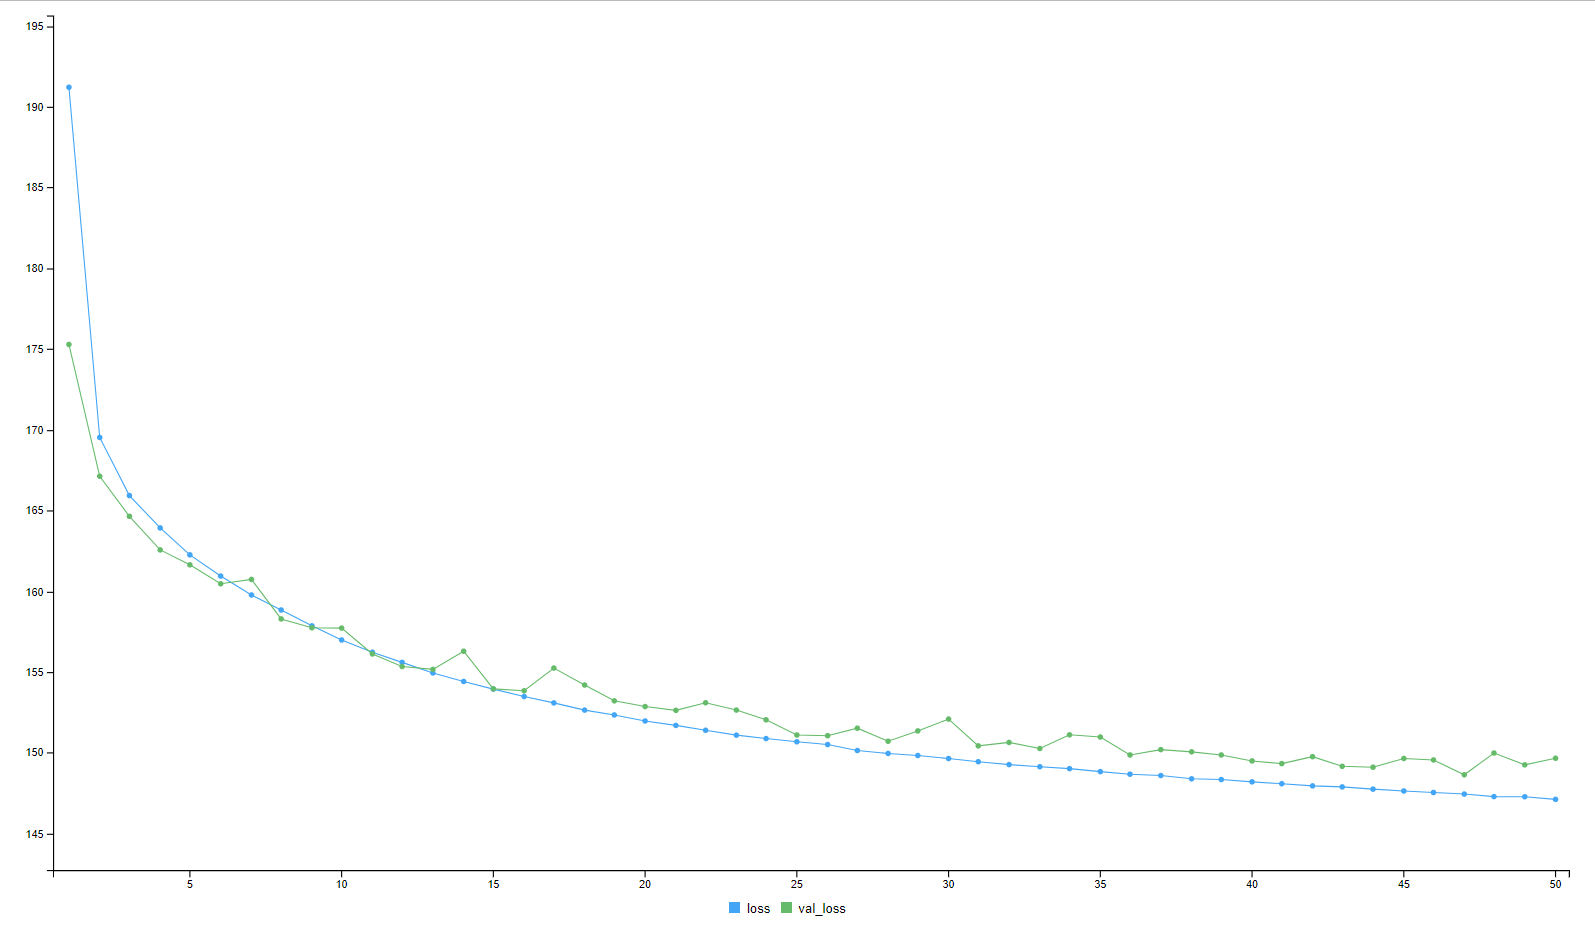
\includegraphics[width=\maxwidth]{vae_hist} \caption[epochs history]{epochs history}\label{fig:unnamed-chunk-7}
\end{figure}

\end{knitrout}

Next plot latent state for the different numbers.
\begin{knitrout}
\definecolor{shadecolor}{rgb}{0.969, 0.969, 0.969}\color{fgcolor}\begin{kframe}
\begin{alltt}
\hlstd{x_test_encoded} \hlkwb{<-} \hlkwd{predict}\hlstd{(encoder, x_test,} \hlkwc{batch_size} \hlstd{= batch_size)}

\hlstd{x_test_encoded} \hlopt
  \hlkwd{as_data_frame}\hlstd{()} \hlopt
  \hlkwd{mutate}\hlstd{(}\hlkwc{class} \hlstd{=} \hlkwd{as.factor}\hlstd{(mnist}\hlopt{$}\hlstd{test}\hlopt{$}\hlstd{y))} \hlopt
  \hlkwd{ggplot}\hlstd{(}\hlkwd{aes}\hlstd{(}\hlkwc{x} \hlstd{= V1,} \hlkwc{y} \hlstd{= V2,} \hlkwc{colour} \hlstd{= class))} \hlopt{+} \hlkwd{geom_point}\hlstd{()}
\end{alltt}
\end{kframe}
\end{knitrout}


\begin{knitrout}
\definecolor{shadecolor}{rgb}{0.969, 0.969, 0.969}\color{fgcolor}\begin{kframe}
\begin{alltt}
\hlstd{knitr}\hlopt{::}\hlkwd{include_graphics}\hlstd{(}\hlstr{"vae_scatter.png"}\hlstd{)}
\end{alltt}
\end{kframe}\begin{figure}
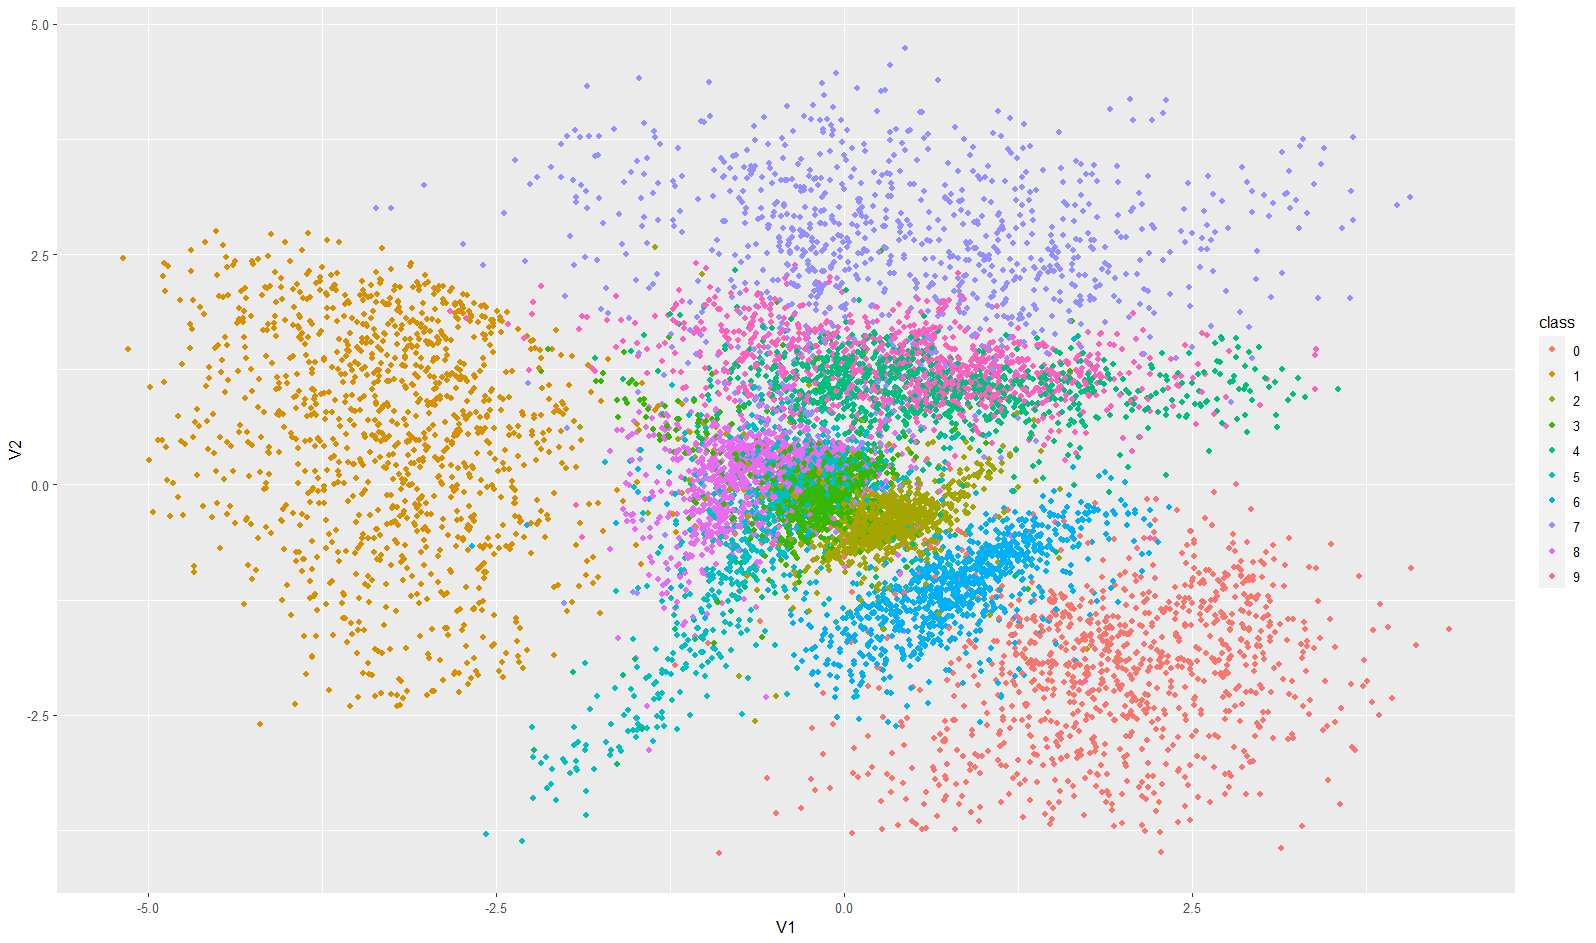
\includegraphics[width=\maxwidth]{vae_scatter} \caption[latent states for different numbers]{latent states for different numbers}\label{fig:unnamed-chunk-9}
\end{figure}

\end{knitrout}

As can be seen from the output. This scatter plot shows how the different classes (digits) are distributed for the hidden states. In general the classes that are close to each other and clustered are better represented, whereas big overlaps means that it is not as good represented. Looking at the plot, then we can see for example that the digit 2 is very centered in the middle and thus well represented, whereas for example the digit 1 is more spread out on the left and not as well represented. 

\subsection{1.5}
Now to encode all the 2s in the test dataset to the latent state using the encoder.

\begin{knitrout}
\definecolor{shadecolor}{rgb}{0.969, 0.969, 0.969}\color{fgcolor}\begin{kframe}
\begin{alltt}
\hlstd{x_digit_2} \hlkwb{<-} \hlstd{x_test[mnist}\hlopt{$}\hlstd{test}\hlopt{$}\hlstd{y} \hlopt{==} \hlnum{2}\hlstd{, ,} \hlkwc{drop} \hlstd{=} \hlnum{FALSE}\hlstd{]}
\hlstd{digit_2_LS} \hlkwb{<-} \hlkwd{predict}\hlstd{(encoder, x_digit_2)}
\hlstd{latent_states_mean} \hlkwb{<-} \hlkwd{colMeans}\hlstd{(digit_2_LS)}
\hlstd{latent_states_mean}
\end{alltt}
\begin{verbatim}
[1]  0.1862775 -0.4990619
\end{verbatim}
\end{kframe}
\end{knitrout}

\subsection{1.6}
And lastly we plot this as an image using the decoder.
\begin{knitrout}
\definecolor{shadecolor}{rgb}{0.969, 0.969, 0.969}\color{fgcolor}\begin{kframe}
\begin{alltt}
\hlkwd{matrix}\hlstd{(latent_states_mean,} \hlkwc{nrow}\hlstd{=}\hlnum{1}\hlstd{)} \hlopt
  \hlkwd{predict}\hlstd{(generator, .)} \hlopt
  \hlkwd{array_reshape}\hlstd{(}\hlkwc{dim}\hlstd{=}\hlkwd{c}\hlstd{(}\hlnum{28}\hlstd{,}\hlnum{28}\hlstd{),} \hlkwc{order} \hlstd{=} \hlkwd{c}\hlstd{(}\hlstr{"F"}\hlstd{))} \hlopt
  \hlkwd{image}\hlstd{(.,} \hlkwc{col} \hlstd{=} \hlkwd{gray.colors}\hlstd{(}\hlkwc{n} \hlstd{=}  \hlnum{256}\hlstd{))}
\end{alltt}
\end{kframe}
\end{knitrout}

\begin{knitrout}
\definecolor{shadecolor}{rgb}{0.969, 0.969, 0.969}\color{fgcolor}\begin{figure}
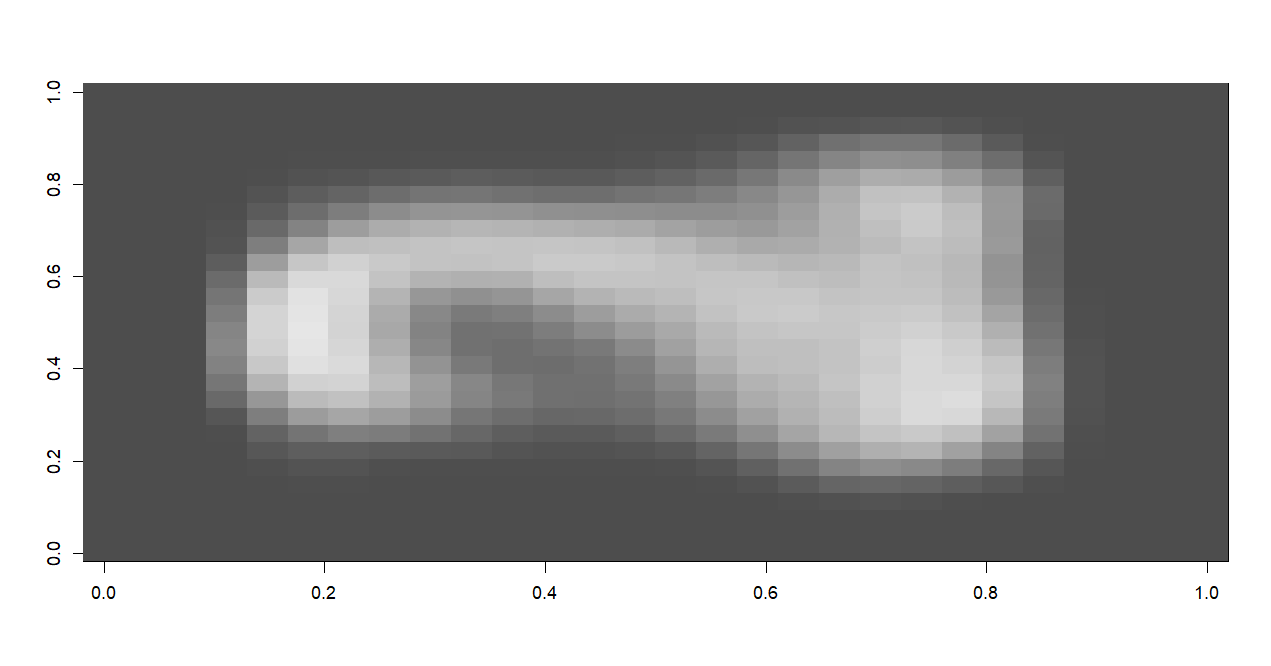
\includegraphics[width=\maxwidth]{mean_latent_img} \caption[28 x 28 pixel image of the latent state]{28 x 28 pixel image of the latent state}\label{fig:unnamed-chunk-12}
\end{figure}

\end{knitrout}


\section{Task 2}
\subsection{2.1}
First we load the data and remove the stopwords.
\begin{knitrout}
\definecolor{shadecolor}{rgb}{0.969, 0.969, 0.969}\color{fgcolor}\begin{kframe}
\begin{alltt}
\hlkwd{library}\hlstd{(uuml)}
\hlkwd{library}\hlstd{(dplyr)}
\hlkwd{library}\hlstd{(tidytext)}
\hlkwd{data}\hlstd{(}\hlstr{"pride_and_prejudice"}\hlstd{)}
\hlkwd{data}\hlstd{(}\hlstr{"stopwords"}\hlstd{)}
\end{alltt}
\end{kframe}
\end{knitrout}

\begin{knitrout}
\definecolor{shadecolor}{rgb}{0.969, 0.969, 0.969}\color{fgcolor}\begin{kframe}
\begin{alltt}
\hlstd{pap} \hlkwb{<-} \hlstd{pride_and_prejudice}
\hlstd{pap} \hlkwb{<-} \hlkwd{anti_join}\hlstd{(pap,} \hlkwc{y} \hlstd{= stopwords[stopwords}\hlopt{$}\hlstd{lexicon} \hlopt{==} \hlstr{"snowball"}\hlstd{,])}
\hlcom{## Joining with `by = join_by(word)`}
\end{alltt}
\end{kframe}
\end{knitrout}

\subsection{2.2}
Next we remove rare words
\begin{knitrout}
\definecolor{shadecolor}{rgb}{0.969, 0.969, 0.969}\color{fgcolor}\begin{kframe}
\begin{alltt}
\hlstd{word_freq} \hlkwb{<-} \hlkwd{table}\hlstd{(pap}\hlopt{$}\hlstd{word)}
\hlstd{rare_words} \hlkwb{<-} \hlkwd{data.frame}\hlstd{(}\hlkwc{word} \hlstd{=} \hlkwd{names}\hlstd{(word_freq[word_freq} \hlopt{<=} \hlnum{5}\hlstd{]),}
                         \hlkwc{stringsAsFactors} \hlstd{=} \hlnum{FALSE}\hlstd{)}
\hlstd{pap} \hlkwb{<-} \hlkwd{anti_join}\hlstd{(pap,} \hlkwc{y} \hlstd{= rare_words)}
\hlcom{## Joining with `by = join_by(word)`}
\end{alltt}
\end{kframe}
\end{knitrout}

\subsection{2.3}

Now to compute a document term matrix where each paragraph is treated as a document. 
\begin{knitrout}
\definecolor{shadecolor}{rgb}{0.969, 0.969, 0.969}\color{fgcolor}\begin{kframe}
\begin{alltt}
\hlkwd{library}\hlstd{(tm)}
\hlstd{crp} \hlkwb{<-} \hlkwd{aggregate}\hlstd{(pap}\hlopt{$}\hlstd{word,} \hlkwc{by} \hlstd{=} \hlkwd{list}\hlstd{(pap}\hlopt{$}\hlstd{paragraph),} \hlkwc{FUN} \hlstd{= paste0,} \hlkwc{collapse} \hlstd{=} \hlstr{" "} \hlstd{)}
\hlkwd{names}\hlstd{(crp)} \hlkwb{<-} \hlkwd{c}\hlstd{(}\hlstr{"paragraph"}\hlstd{,} \hlstr{"text"}\hlstd{)}
\hlstd{s} \hlkwb{<-} \hlkwd{SimpleCorpus}\hlstd{(}\hlkwd{VectorSource}\hlstd{(crp}\hlopt{$}\hlstd{text))}
\hlstd{m} \hlkwb{<-} \hlkwd{DocumentTermMatrix}\hlstd{(s)}
\hlkwd{print}\hlstd{(s)}
\end{alltt}
\begin{verbatim}
<<SimpleCorpus>>
Metadata:  corpus specific: 1, document level (indexed): 0
Content:  documents: 2051
\end{verbatim}
\begin{alltt}
\hlkwd{print}\hlstd{(m)}
\end{alltt}
\begin{verbatim}
<<DocumentTermMatrix (documents: 2051, terms: 1689)>>
Non-/sparse entries: 42130/3422009
Sparsity           : 99%
Maximal term length: 15
Weighting          : term frequency (tf)
\end{verbatim}
\end{kframe}
\end{knitrout}
Here we have 2051 documents and 1689 terms.

\subsection{2.4}
For this step we runt the Gibbs sampler for 2000 iterations.
\begin{knitrout}
\definecolor{shadecolor}{rgb}{0.969, 0.969, 0.969}\color{fgcolor}\begin{kframe}
\begin{alltt}
\hlkwd{library}\hlstd{(topicmodels)}
\hlstd{K} \hlkwb{<-} \hlnum{10}
\hlstd{control} \hlkwb{<-} \hlkwd{list}\hlstd{(}\hlkwc{keep} \hlstd{=} \hlnum{1}\hlstd{,} \hlkwc{delta} \hlstd{=} \hlnum{0.1}\hlstd{,} \hlkwc{alpha} \hlstd{=} \hlnum{1}\hlstd{,} \hlkwc{iter} \hlstd{=} \hlnum{2000}\hlstd{)}
\hlstd{tm} \hlkwb{<-} \hlkwd{LDA}\hlstd{(m,} \hlkwc{k} \hlstd{= K,} \hlkwc{method} \hlstd{=} \hlstr{"Gibbs"}\hlstd{, control)}
\end{alltt}
\end{kframe}
\end{knitrout}

\subsection{2.5}

Next we extract some parameters.

\begin{knitrout}
\definecolor{shadecolor}{rgb}{0.969, 0.969, 0.969}\color{fgcolor}\begin{kframe}
\begin{alltt}
\hlstd{lls} \hlkwb{<-} \hlkwd{extract_log_liks}\hlstd{(tm)}
\hlstd{theta} \hlkwb{<-} \hlkwd{extract_theta}\hlstd{(tm)}
\hlstd{phi} \hlkwb{<-} \hlkwd{extract_phi}\hlstd{(tm)}
\end{alltt}
\end{kframe}
\end{knitrout}


\subsection{2.6}
And now to check if the log likelihood has converged.
\begin{knitrout}
\definecolor{shadecolor}{rgb}{0.969, 0.969, 0.969}\color{fgcolor}\begin{kframe}
\begin{alltt}
\hlkwd{plot}\hlstd{(lls,} \hlkwc{ylab}\hlstd{=}\hlstr{"Log-likelihood"}\hlstd{,} \hlkwc{xlab}\hlstd{=}\hlstr{"Epoch"}\hlstd{)}
\end{alltt}
\end{kframe}\begin{figure}
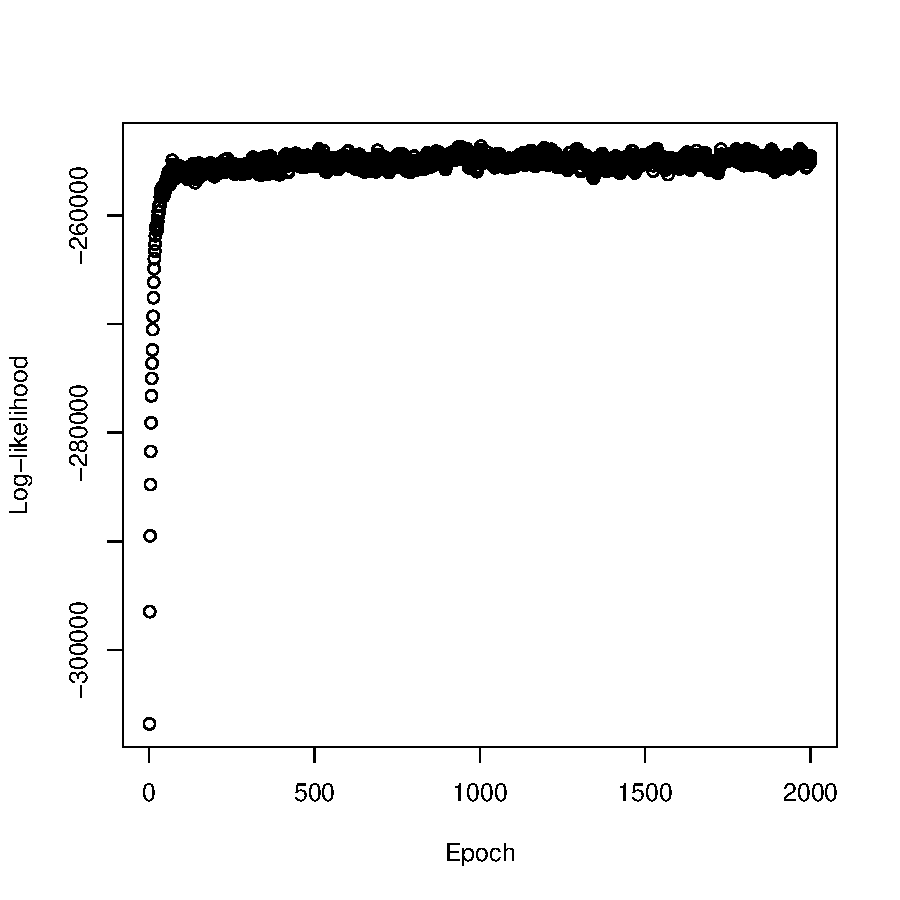
\includegraphics[width=\maxwidth]{figure/unnamed-chunk-19-1} \caption[Log likelihood for epochs]{Log likelihood for epochs}\label{fig:unnamed-chunk-19}
\end{figure}

\end{knitrout}
Looking at the figure, it seems as if the log-likelihood has converged. 
\subsection{2.7}
Now we extract the top 20 words for each of the 10 topic.
\begin{knitrout}
\definecolor{shadecolor}{rgb}{0.969, 0.969, 0.969}\color{fgcolor}\begin{kframe}
\begin{alltt}
\hlcom{#function to extract n number of top words given topic}
\hlstd{extract_func} \hlkwb{<-} \hlkwa{function}\hlstd{(}\hlkwc{topic_index}\hlstd{,} \hlkwc{phi_parameter}\hlstd{,} \hlkwc{n_words}\hlstd{)\{}
  \hlstd{words} \hlkwb{<-} \hlkwd{colnames}\hlstd{(phi_parameter)[}\hlkwd{order}\hlstd{(}\hlopt{-}\hlstd{phi_parameter[topic_index,])]}
  \hlkwd{return}\hlstd{(words[}\hlnum{1}\hlopt{:}\hlstd{n_words])}
\hlstd{\}}

\hlcom{#using the function over all 10 topics}
\hlkwd{sapply}\hlstd{(}\hlnum{1}\hlopt{:}\hlnum{10}\hlstd{,} \hlkwc{FUN} \hlstd{=}\hlkwa{function}\hlstd{(}\hlkwc{i}\hlstd{)\{}\hlkwd{extract_func}\hlstd{(}\hlkwc{topic_index}\hlstd{=i,} \hlkwc{phi_parameter} \hlstd{= phi,} \hlkwc{n_words}\hlstd{=}\hlnum{20}\hlstd{)\})}
\end{alltt}
\begin{verbatim}
      [,1]        [,2]        [,3]      [,4]          [,5]          [,6]     
 [1,] "now"       "lady"      "lydia"   "mrs"         "elizabeth"   "will"   
 [2,] "letter"    "collins"   "good"    "bennet"      "darcy"       "can"    
 [3,] "nothing"   "catherine" "wickham" "day"         "said"        "may"    
 [4,] "soon"      "great"     "well"    "two"         "made"        "shall"  
 [5,] "wickham"   "sir"       "never"   "soon"        "little"      "know"   
 [6,] "give"      "charlotte" "said"    "time"        "looked"      "dear"   
 [7,] "without"   "time"      "know"    "morning"     "manner"      "said"   
 [8,] "done"      "lucas"     "mother"  "longbourn"   "speak"       "say"    
 [9,] "first"     "first"     "aunt"    "next"        "answer"      "think"  
[10,] "ill"       "make"      "sure"    "till"        "eyes"        "must"   
[11,] "present"   "young"     "kitty"   "netherfield" "might"       "lizzy"  
[12,] "known"     "rosings"   "father"  "went"        "pemberley"   "one"    
[13,] "since"     "way"       "gone"    "daughters"   "spoke"       "believe"
[14,] "last"      "family"    "away"    "might"       "mind"        "yes"    
[15,] "received"  "little"    "meryton" "husband"     "felt"        "let"    
[16,] "knew"      "daughter"  "going"   "home"        "continued"   "hope"   
[17,] "long"      "however"   "now"     "leave"       "elizabeth's" "replied"
[18,] "hardly"    "much"      "place"   "coming"      "without"     "well"   
[19,] "therefore" "cousin"    "married" "family"      "whether"     "indeed" 
[20,] "told"      "william"   "thought" "added"       "last"        "upon"   
      [,7]        [,8]        [,9]        [,10]         
 [1,] "miss"      "man"       "must"      "elizabeth"   
 [2,] "bingley"   "never"     "every"     "room"        
 [3,] "darcy"     "think"     "elizabeth" "house"       
 [4,] "jane"      "good"      "might"     "said"        
 [5,] "much"      "always"    "though"    "mrs"         
 [6,] "sister"    "young"     "happiness" "saw"         
 [7,] "elizabeth" "many"      "less"      "every"       
 [8,] "friend"    "world"     "affection" "party"       
 [9,] "though"    "much"      "make"      "ladies"      
[10,] "enough"    "must"      "love"      "soon"        
[11,] "see"       "father"    "still"     "began"       
[12,] "nothing"   "life"      "marriage"  "conversation"
[13,] "two"       "anything"  "yet"       "walk"        
[14,] "bingley's" "ever"      "almost"    "took"        
[15,] "one"       "little"    "without"   "walked"      
[16,] "sisters"   "manners"   "happy"     "towards"     
[17,] "say"       "means"     "really"    "turned"      
[18,] "well"      "pride"     "hope"      "civility"    
[19,] "however"   "often"     "regard"    "door"        
[20,] "asked"     "agreeable" "wish"      "entered"     
\end{verbatim}
\end{kframe}
\end{knitrout}

Looking at the topics, then I would say that perhaps topic 1 since it contains some words that reflects some key concepts and general state of the novel. For example, that the idea is the everyone must find someone to marry in order to bring happiness, but in the process of doing so the sisters reflect on the situation and general feelings on whether or not they actually want to go thorugh with it or not . Annother topic is perhaps topic 4 since it contains some of the names of the characters in the novel, or the relationships between the chaaracetsr suc has bennet, bingley,  Elizabeth or netherfield, as well as some descriptions such as daughters, sisters or mother and so on. 
\subsection{2.8}
Next we visualize how these evolve over the paragraphs.
\begin{knitrout}
\definecolor{shadecolor}{rgb}{0.969, 0.969, 0.969}\color{fgcolor}\begin{kframe}
\begin{alltt}
\hlstd{plot_topics} \hlkwb{<-} \hlkwa{function}\hlstd{(}\hlkwc{theta_matrix}\hlstd{,} \hlkwc{col_index1}\hlstd{,} \hlkwc{col_index2}\hlstd{) \{}
  \hlstd{paragraphs} \hlkwb{<-} \hlnum{1}\hlopt{:}\hlkwd{nrow}\hlstd{(theta_matrix)}
  \hlstd{topic1} \hlkwb{<-} \hlstd{theta_matrix[, col_index1]}
  \hlstd{topic2} \hlkwb{<-} \hlstd{theta_matrix[, col_index2]}

  \hlstd{new_df} \hlkwb{<-} \hlkwd{tibble}\hlstd{(paragraphs, topic1, topic2)}
  \hlstd{name1} \hlkwb{<-} \hlkwd{paste}\hlstd{(}\hlstr{"Topic no. "}\hlstd{, col_index1)}
  \hlstd{name2} \hlkwb{<-} \hlkwd{paste}\hlstd{(}\hlstr{"Topic no. "}\hlstd{, col_index2)}

  \hlstd{new_df} \hlopt
    \hlkwd{ggplot}\hlstd{(}\hlkwd{aes}\hlstd{(}\hlkwc{x} \hlstd{= paragraphs))} \hlopt{+}
    \hlkwd{geom_line}\hlstd{(}\hlkwd{aes}\hlstd{(}\hlkwc{y} \hlstd{= topic1,} \hlkwc{color} \hlstd{= name1),} \hlkwc{size} \hlstd{=} \hlnum{1}\hlstd{)} \hlopt{+}
    \hlkwd{geom_line}\hlstd{(}\hlkwd{aes}\hlstd{(}\hlkwc{y} \hlstd{= topic2,} \hlkwc{color} \hlstd{= name2),} \hlkwc{size} \hlstd{=} \hlnum{1}\hlstd{)} \hlopt{+}
     \hlkwd{scale_color_discrete}\hlstd{(}\hlkwc{name}\hlstd{=}\hlstr{""}\hlstd{)} \hlopt{+}
    \hlkwd{labs}\hlstd{(}
      \hlkwc{title} \hlstd{=} \hlstr{"Topics over time on paragraphs"}\hlstd{,}
      \hlkwc{x} \hlstd{=} \hlstr{"Paragraph"}\hlstd{,}
      \hlkwc{y} \hlstd{=} \hlkwd{expression}\hlstd{(theta)}
    \hlstd{)}
\hlstd{\}}

\hlkwd{plot_topics}\hlstd{(theta,} \hlnum{1}\hlstd{,} \hlnum{4}\hlstd{)}
\end{alltt}
\end{kframe}\begin{figure}
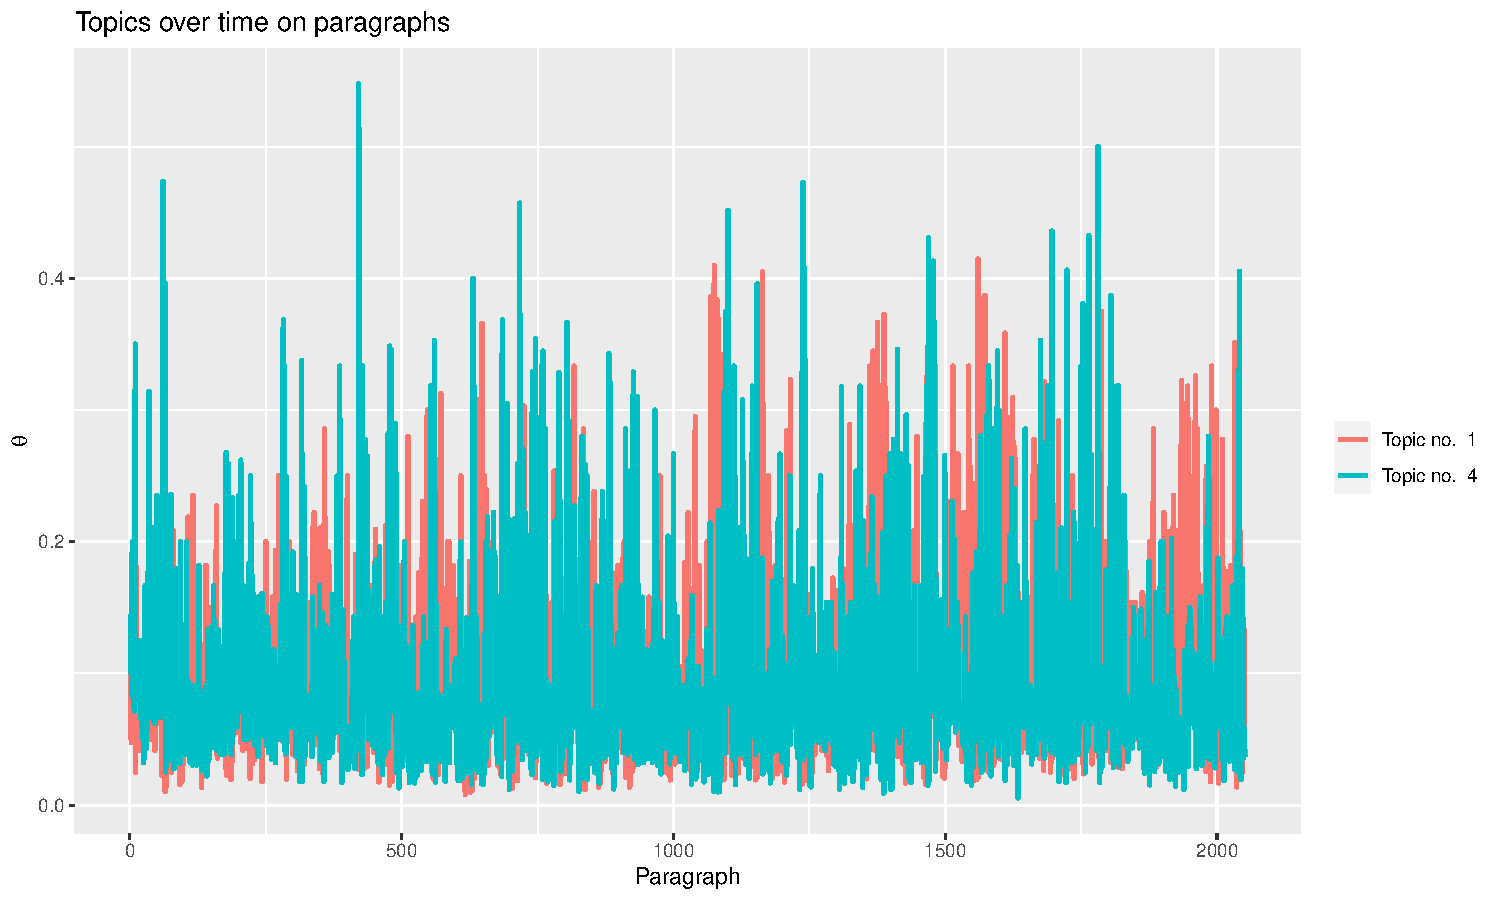
\includegraphics[width=\maxwidth]{figure/unnamed-chunk-21-1} \caption[vizualisation of topics over time]{vizualisation of topics over time}\label{fig:unnamed-chunk-21}
\end{figure}

\end{knitrout}

\subsection{2.9}
Lastly, we visualize it again as a rolling mean with k=5. 
\begin{knitrout}
\definecolor{shadecolor}{rgb}{0.969, 0.969, 0.969}\color{fgcolor}\begin{kframe}
\begin{alltt}
\hlkwd{head}\hlstd{(zoo}\hlopt{::}\hlkwd{rollmean}\hlstd{(theta[,}\hlnum{1}\hlstd{],} \hlkwc{k}\hlstd{=}\hlnum{5}\hlstd{))}
\end{alltt}
\begin{verbatim}
         3          4          5          6          7          8 
0.09142857 0.09681319 0.08157509 0.08633700 0.10300366 0.08133700 
\end{verbatim}
\begin{alltt}
\hlstd{theta_rolling_m} \hlkwb{<-} \hlstd{zoo}\hlopt{::}\hlkwd{rollmean}\hlstd{(}\hlkwc{x}\hlstd{=theta,} \hlkwc{k} \hlstd{=}\hlnum{5}\hlstd{)}
\hlkwd{plot_topics}\hlstd{(theta_rolling_m,} \hlnum{1}\hlstd{,} \hlnum{4}\hlstd{)}
\end{alltt}
\end{kframe}\begin{figure}
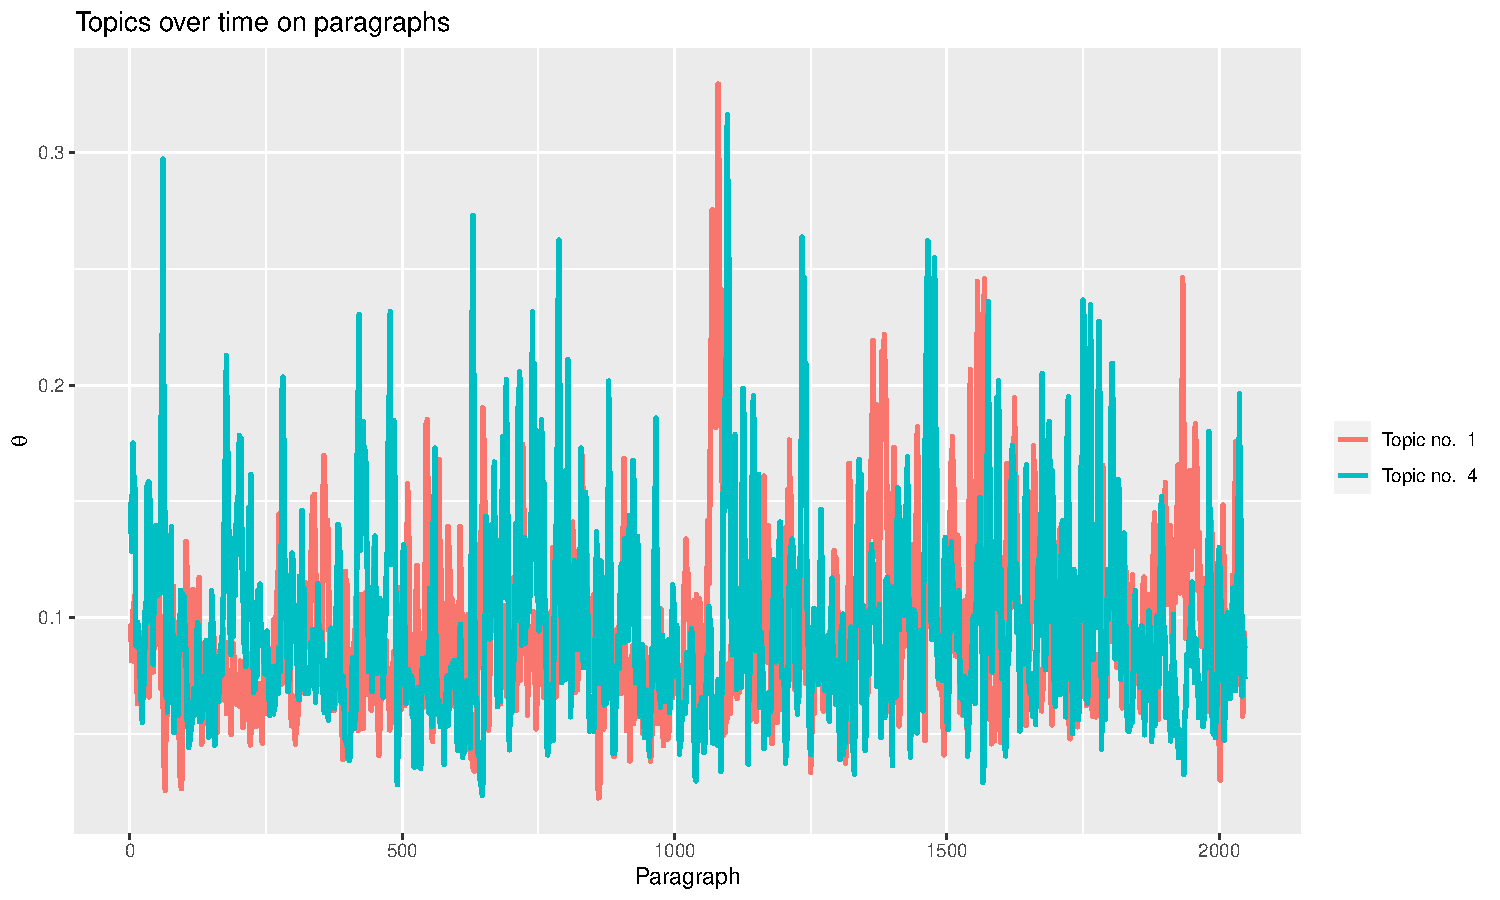
\includegraphics[width=\maxwidth]{figure/topic_means-1} \caption[Topic rolling means]{Topic rolling means}\label{fig:topic_means}
\end{figure}

\end{knitrout}
Looking as this figure, we see that in general Topic number 4 seems to always somewhat relevant for the different paragraphs such that we see the value for theta jumping back and fort between 0.5 - 0.25, but it does so somewhat consistently across the different paragraphs, albeit there being a decrease in the middle for a short while. Looking at topic number 1 , we see that it is not as prevalent in the first quarter of the paragraphs, but then evolves to be more relevant in the middle and the end , which perhaps can be attributed due to the fact that it contained many names that becomes more relevant during that period. 

\end{document}
